\section{Graphs and Plots}

\subsection{2D Plots}
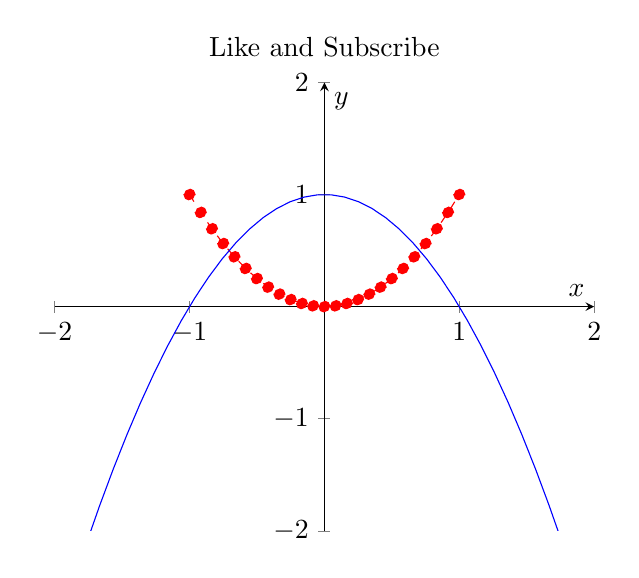
\begin{tikzpicture}
    \begin{axis}[xmin=-2,
            xmax=2,
            ymin=-2,
            ymax=2,
            axis lines = middle,
            xlabel=$x$,
            ylabel=$y$,
            title={Like and Subscribe}]
        \addplot[color=red, dashed, mark=*, samples=25, domain=-1:1]{x^2};
        \addplot[color=blue, samples=100]{1-x^2};
    \end{axis}
\end{tikzpicture}

\vspace{1in}

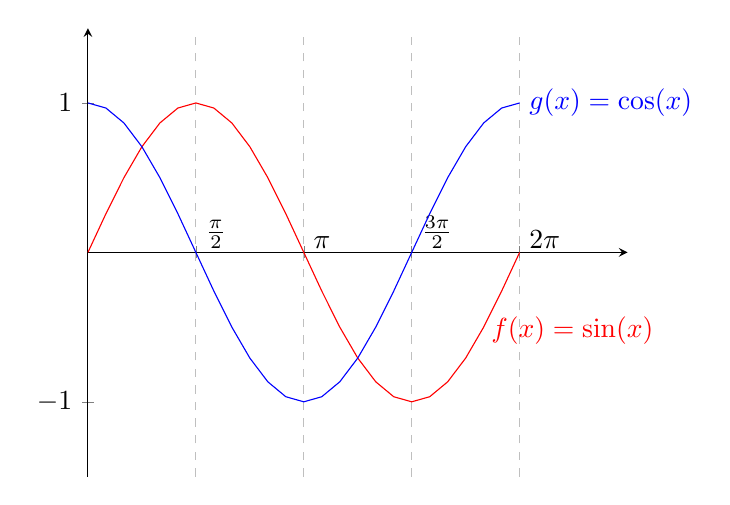
\begin{tikzpicture}
    \begin{axis}[clip=false,
            xmin=0,xmax=2.5*pi,
            ymin=-1.5,ymax=1.5,
            axis lines = middle,
            xtick={0,pi/2,pi,3*pi/2,2*pi},
            xticklabels={0, $\frac{\pi}{2}$, $\pi$, $\frac{3\pi}{2}$, $2\pi$},
            xticklabel style={anchor=south west},
            xmajorgrids=true,
            grid style=dashed]
        \addplot[domain=0:2*pi,red]{sin(deg(x))} node[right,pos=0.9]{$f(x) = \sin(x)$};
        \addplot[domain=0:2*pi,blue]{cos(deg(x))} node[right,pos=1]{$g(x) = \cos(x)$};
    \end{axis}
\end{tikzpicture}

\vspace{1in}

\begin{tikzpicture}
    \begin{axis}
        \addplot +[only marks, scatter, mark size = 2.9pt] %'+' adds extra formatting on top of the default. This says to only show the points, don't draw lines - and also defines the mark size and style as 'scatter'
        table[meta=ma]{Data/text.txt}; %Imports the data from the file
    \end{axis}
\end{tikzpicture}

\begin{tikzpicture}
    \begin{axis}[scatter/classes={
                    a={mark=square*,blue},
                    b={mark=triangle*,red},
                    c={mark=o,draw=black}
                }]
        \addplot[scatter, only marks, scatter src = explicit symbolic]
        coordinates {
                (0.1,0.15) [a]
                (0.45,0.27) [c]
                (0.02,0.17) [a]
                (0.06,0.1) [a]
                (0.9,0.5) [b]
                (0.5,0.3) [c]
                (0.85,0.52) [b]
                (0.12,0.05) [a]
                (0.73,0.45) [b]
                (0.53,0.25) [c]
                (0.76,0.5) [b]
                (0.55,0.32) [c]
            };
    \end{axis}
\end{tikzpicture}


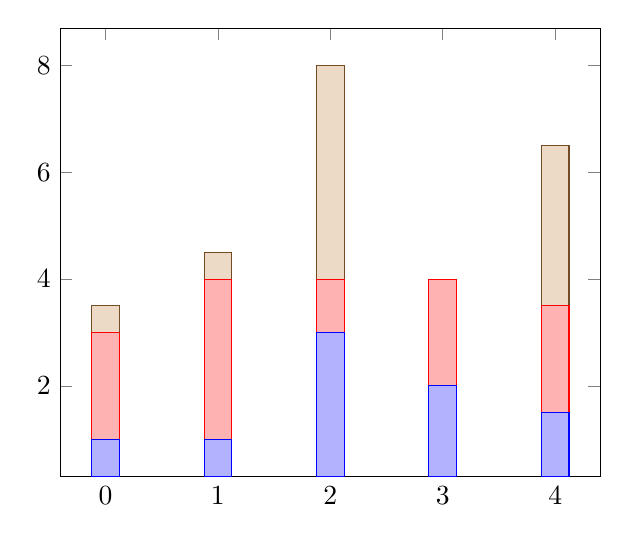
\begin{tikzpicture}
    \begin{axis}[ybar stacked]
        \addplot coordinates
            {(0,1) (1,1) (2,3) (3,2) (4,1.5)};
        \addplot coordinates
            {(0,2) (1,3) (2,1) (3,2) (4,2)};
        \addplot coordinates
            {(0,0.5) (1,0.5) (2,4) (3,0) (4,3)};
    \end{axis}
\end{tikzpicture}

\newpage

\subsection{3D Plots}
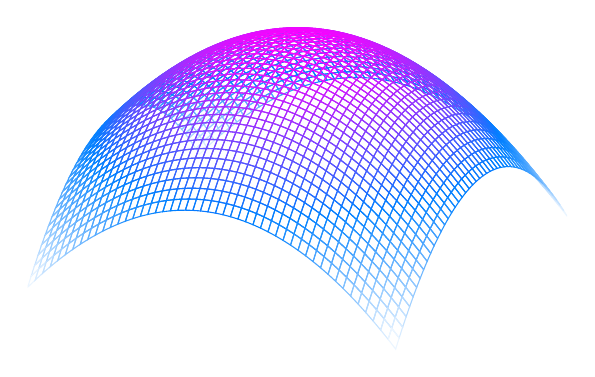
\begin{tikzpicture}
    \begin{axis}[colormap/cool,
            hide axis]
        \addplot3[mesh, samples=50]{1-x^2-y^2}; % use surf and shader=interp for smooth surface with no squares
    \end{axis}
\end{tikzpicture}

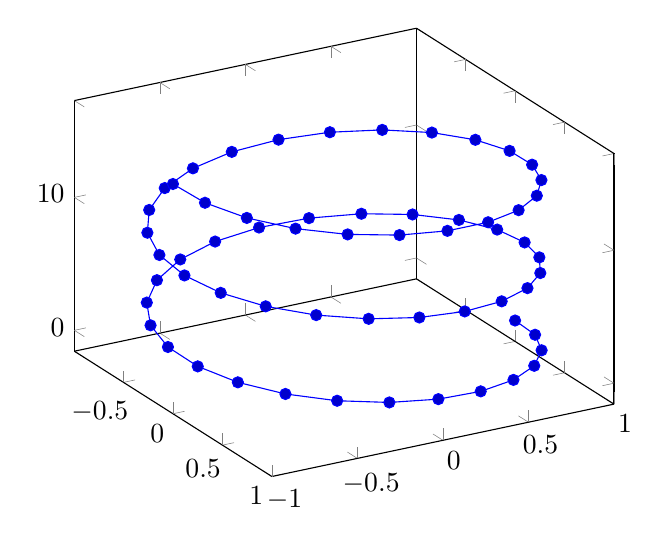
\begin{tikzpicture}
    \begin{axis}[view={60}{30}]
        \addplot3+[domain=0:5*pi, samples=60, samples y=0]
        ({sin(deg(x))},
        {cos(deg(x))},
        {x});
    \end{axis}
\end{tikzpicture}